\documentclass[10pt,a4paper]{article}
\usepackage[T1]{fontenc}
\usepackage[margin=1.8cm]{geometry}
\usepackage{underscore}
\usepackage{longtable,booktabs,array,graphicx}
\usepackage{tikz}
\usepackage{pdflscape}
\usetikzlibrary{arrows.meta,positioning,calc}
\setlength{\parindent}{0pt}
\setlength{\parskip}{4pt}

\begin{document}

{\LARGE\bfseries Tiny FPGA LM: inference FSM and parallel MAC lanes}

\medskip
Arty A7-100T, 100 MHz. One FSM sequences the embedding lookup, both fully connected layers, and the argmax.
The same 8-lane MAC array and the same states serve both layers; only the \texttt{output_layer} register changes.

\section*{1. Inference FSM}

\begin{center}
\resizebox{\textwidth}{!}{%
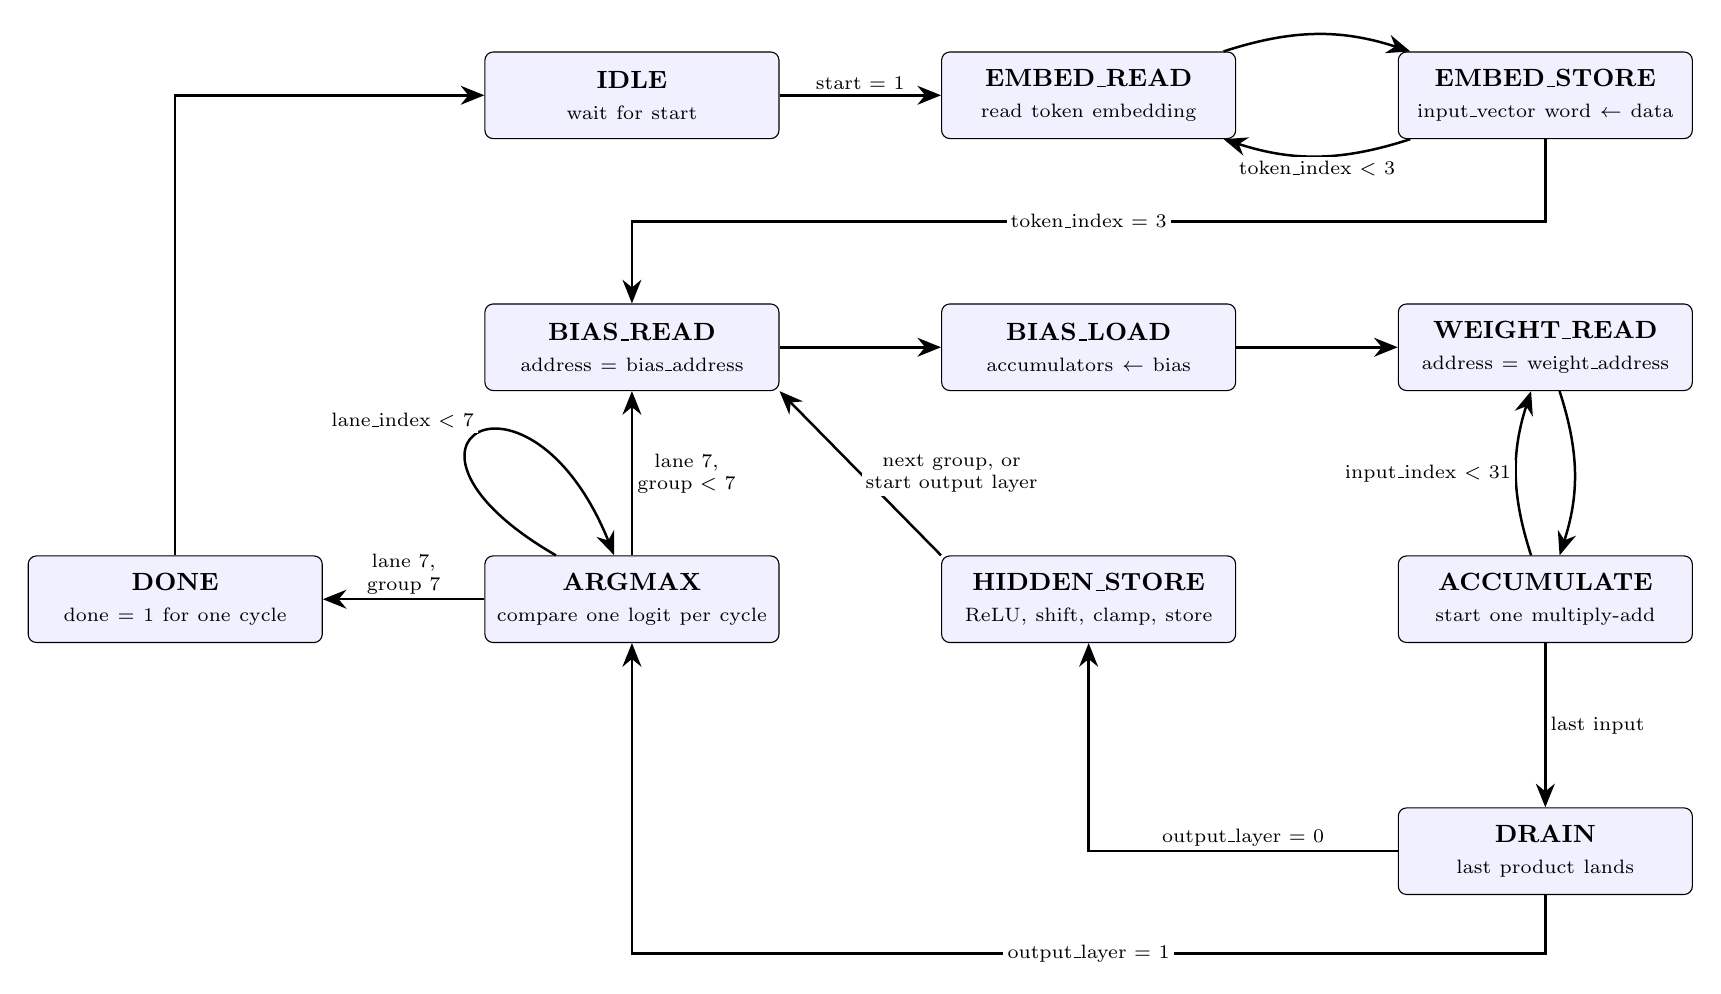
\begin{tikzpicture}[>={Stealth[length=3mm,width=2.4mm]},
  state/.style={draw,rounded corners=3pt,minimum width=3.7cm,minimum height=1.1cm,
                align=center,fill=blue!6,text width=3.5cm,font=\small},
  tr/.style={->,line width=0.9pt},
  lab/.style={font=\scriptsize,fill=white,inner sep=1.5pt,align=center}]

\node[state] (idle) at (0,0)     {\textbf{IDLE}\\{\scriptsize wait for start}};
\node[state] (er)   at (5.8,0)   {\textbf{EMBED_READ}\\{\scriptsize read token embedding}};
\node[state] (es)   at (11.6,0)  {\textbf{EMBED_STORE}\\{\scriptsize input_vector word $\leftarrow$ data}};

\node[state] (br)   at (0,-3.2)    {\textbf{BIAS_READ}\\{\scriptsize address = bias_address}};
\node[state] (bl)   at (5.8,-3.2)  {\textbf{BIAS_LOAD}\\{\scriptsize accumulators $\leftarrow$ bias}};
\node[state] (wr)   at (11.6,-3.2) {\textbf{WEIGHT_READ}\\{\scriptsize address = weight_address}};

\node[state] (am)   at (0,-6.4)    {\textbf{ARGMAX}\\{\scriptsize compare one logit per cycle}};
\node[state] (hs)   at (5.8,-6.4)  {\textbf{HIDDEN_STORE}\\{\scriptsize ReLU, shift, clamp, store}};
\node[state] (acc)  at (11.6,-6.4) {\textbf{ACCUMULATE}\\{\scriptsize start one multiply-add}};
\node[state] (dr)   at (11.6,-9.6) {\textbf{DRAIN}\\{\scriptsize last product lands}};
\node[state] (done) at (-5.8,-6.4) {\textbf{DONE}\\{\scriptsize done = 1 for one cycle}};

\draw[tr] (idle) -- node[above,lab]{start = 1} (er);
\draw[tr] (er) to[bend left=18] (es);
\draw[tr] (es) to[bend left=18] node[below,lab]{token_index $<$ 3} (er);

\draw[tr] (es.south) -- (11.6,-1.6) -- (0,-1.6) -- (br.north);
\node[lab] at (5.8,-1.6) {token_index = 3};

\draw[tr] (br) -- (bl);
\draw[tr] (bl) -- (wr);

\draw[tr] (wr) to[bend left=18] (acc);
\draw[tr] (acc) to[bend left=18] node[left,lab]{input_index $<$ 31} (wr);

\draw[tr] (acc) -- node[right,lab]{last input} (dr);
\draw[tr] (dr.west) -| node[pos=0.25,above,lab]{output_layer = 0} (hs.south);
\draw[tr] (dr.south) -- (11.6,-10.9) -- (0,-10.9) -- (am.south);
\node[lab] at (5.8,-10.9) {output_layer = 1};

\draw[tr] (hs.north west) -- node[right,lab]{next group, or\\start output layer} (br.south east);

\draw[tr] (am) -- node[right,lab]{lane 7,\\group $<$ 7} (br);
\draw[tr] (am.150) to[out=150,in=112,looseness=10] node[above left,lab]{lane_index $<$ 7} (am.112);
\draw[tr] (am) -- node[above,lab]{lane 7,\\group 7} (done);

\draw[tr] (done.north) -- (-5.8,0) -- (idle.west);
\end{tikzpicture}}
\end{center}

\subsection*{State transition table}

\footnotesize
\begin{longtable}{@{}>{\ttfamily}p{2.3cm} >{\ttfamily}p{2.9cm} >{\ttfamily}p{2.3cm} p{8.3cm}@{}}
\toprule
\textbf{State} & \textbf{Condition} & \textbf{Next state} & \textbf{Register updates at the clock edge} \\
\midrule
\endhead
IDLE & start = 0 & IDLE & token_index, group_index, input_index, lane_index, weight_address, bias_address, output_layer $\leftarrow$ 0 (every cycle spent in IDLE); argmax_clear = 1 \\
IDLE & start = 1 & EMBED_READ & same clearing; argmax_clear = 1 holds best_value at $-2^{31}$ and best_index at 0 \\
\midrule
EMBED_READ & always & EMBED_STORE & embedding ROM latches the word at address token[token_index] \\
EMBED_STORE & token_index $<$ 3 & EMBED_READ & input_vector word token_index $\leftarrow$ embedding ROM output (8 $\times$ INT8); token_index $\leftarrow$ token_index + 1 \\
EMBED_STORE & token_index = 3 & BIAS_READ & input_vector word 3 $\leftarrow$ embedding ROM output \\
\midrule
BIAS_READ & always & BIAS_LOAD & bias ROM latches the word at bias_address \\
BIAS_LOAD & always & WEIGHT_READ & accumulator$_i$ $\leftarrow$ bias$_i$ for all 8 lanes; bias_address $\leftarrow$ bias_address + 1 \\
\midrule
WEIGHT_READ & always & ACCUMULATE & weight ROM latches the word at weight_address. The activation is selected from input_vector (output_layer = 0) or hidden_buf (output_layer = 1) using input_index, and mac_array registers it \\
ACCUMULATE & input_index $<$ 31 & WEIGHT_READ & each lane registers activation $\cdot$ weight$_i$; one clock later it adds that product into accumulator$_i$; weight_address $\leftarrow$ weight_address + 1; input_index $\leftarrow$ input_index + 1 \\
ACCUMULATE & input_index = 31 & DRAIN & same multiply-add; input_index $\leftarrow$ 0 \\
DRAIN & output_layer = 0 & HIDDEN_STORE & no register updates: waits one clock so the last product reaches the accumulators \\
DRAIN & output_layer = 1 & ARGMAX & same wait \\
\midrule
HIDDEN_STORE & group_index $<$ 3 & BIAS_READ & hidden_buf byte group $\leftarrow$ clamp(ReLU(accumulator$_i$) $\gg$ 4) for 8 lanes; group_index $\leftarrow$ group_index + 1 \\
HIDDEN_STORE & group_index = 3 & BIAS_READ & same store; output_layer $\leftarrow$ 1; group_index $\leftarrow$ 0 \\
\midrule
ARGMAX & lane_index $<$ 7 & ARGMAX & if accumulator[lane_index] $>$ best_value: best_value $\leftarrow$ it, best_index $\leftarrow$ \{group_index, lane_index\}; lane_index $\leftarrow$ lane_index + 1 \\
ARGMAX & lane_index = 7, group_index $<$ 7 & BIAS_READ & same compare; lane_index wraps from 7 to 0; group_index $\leftarrow$ group_index + 1 \\
ARGMAX & lane_index = 7, group_index = 7 & DONE & same compare \\
\midrule
DONE & always & IDLE & done = 1 this cycle; predicted_token = best_index \\
\bottomrule
\end{longtable}
\normalsize

\subsection*{Registers and memory layout}

\footnotesize
\begin{tabular}{@{}>{\ttfamily}l l p{11cm}@{}}
\toprule
\textbf{Register} & \textbf{Bits} & \textbf{Meaning} \\
\midrule
state & 4 & current FSM state \\
output_layer & 1 & 0 = hidden layer (32$\to$32), 1 = output layer (32$\to$64) \\
token_index & 2 & which of the 4 context tokens is being embedded \\
group_index & 3 & which group of 8 output neurons (0--3 in the hidden layer, 0--7 in the output layer) \\
input_index & 5 & which of the 32 inputs within a group \\
lane_index & 3 & which lane's logit ARGMAX is examining \\
weight_address & 9 & next weight ROM word, 0 to 383; counts up and is not reset between layers \\
bias_address & 4 & next bias ROM word, 0 to 11 \\
best_value & 32 signed & largest logit so far \\
best_index & 6 & token ID of the largest logit so far (the output byte) \\
\bottomrule
\end{tabular}

\medskip
Weight ROM: 384 words of 64 bits (8 $\times$ INT8). Words 0--127 are the hidden layer (word = group$\cdot$32 + input), words 128--383 are the output layer. Because the FSM visits words in order, the address is a plain counter with no multiplier.
Word bits [8i+7:8i] hold $W[8\cdot\mathrm{group}+i][\mathrm{input}]$ and go to lane $i$. The Python weight export must use this ordering.

Bias ROM: 12 words of 256 bits (8 $\times$ INT32), words 0--3 for the hidden layer and 4--11 for the output layer. Embedding ROM: 64 words of 64 bits (8 $\times$ INT8).

Latency: 8 cycles of embedding, 4 $\times$ 68 cycles for the hidden layer, 8 $\times$ 75 for the output layer, plus DONE, 881 cycles or 8.8 $\mu$s. One UART byte at 115200 baud takes 87 $\mu$s, so the sequencing cost is negligible.
\normalsize

\begin{landscape}
\section*{2. Eight parallel MAC lanes}

\begin{center}
\resizebox{\textwidth}{!}{%
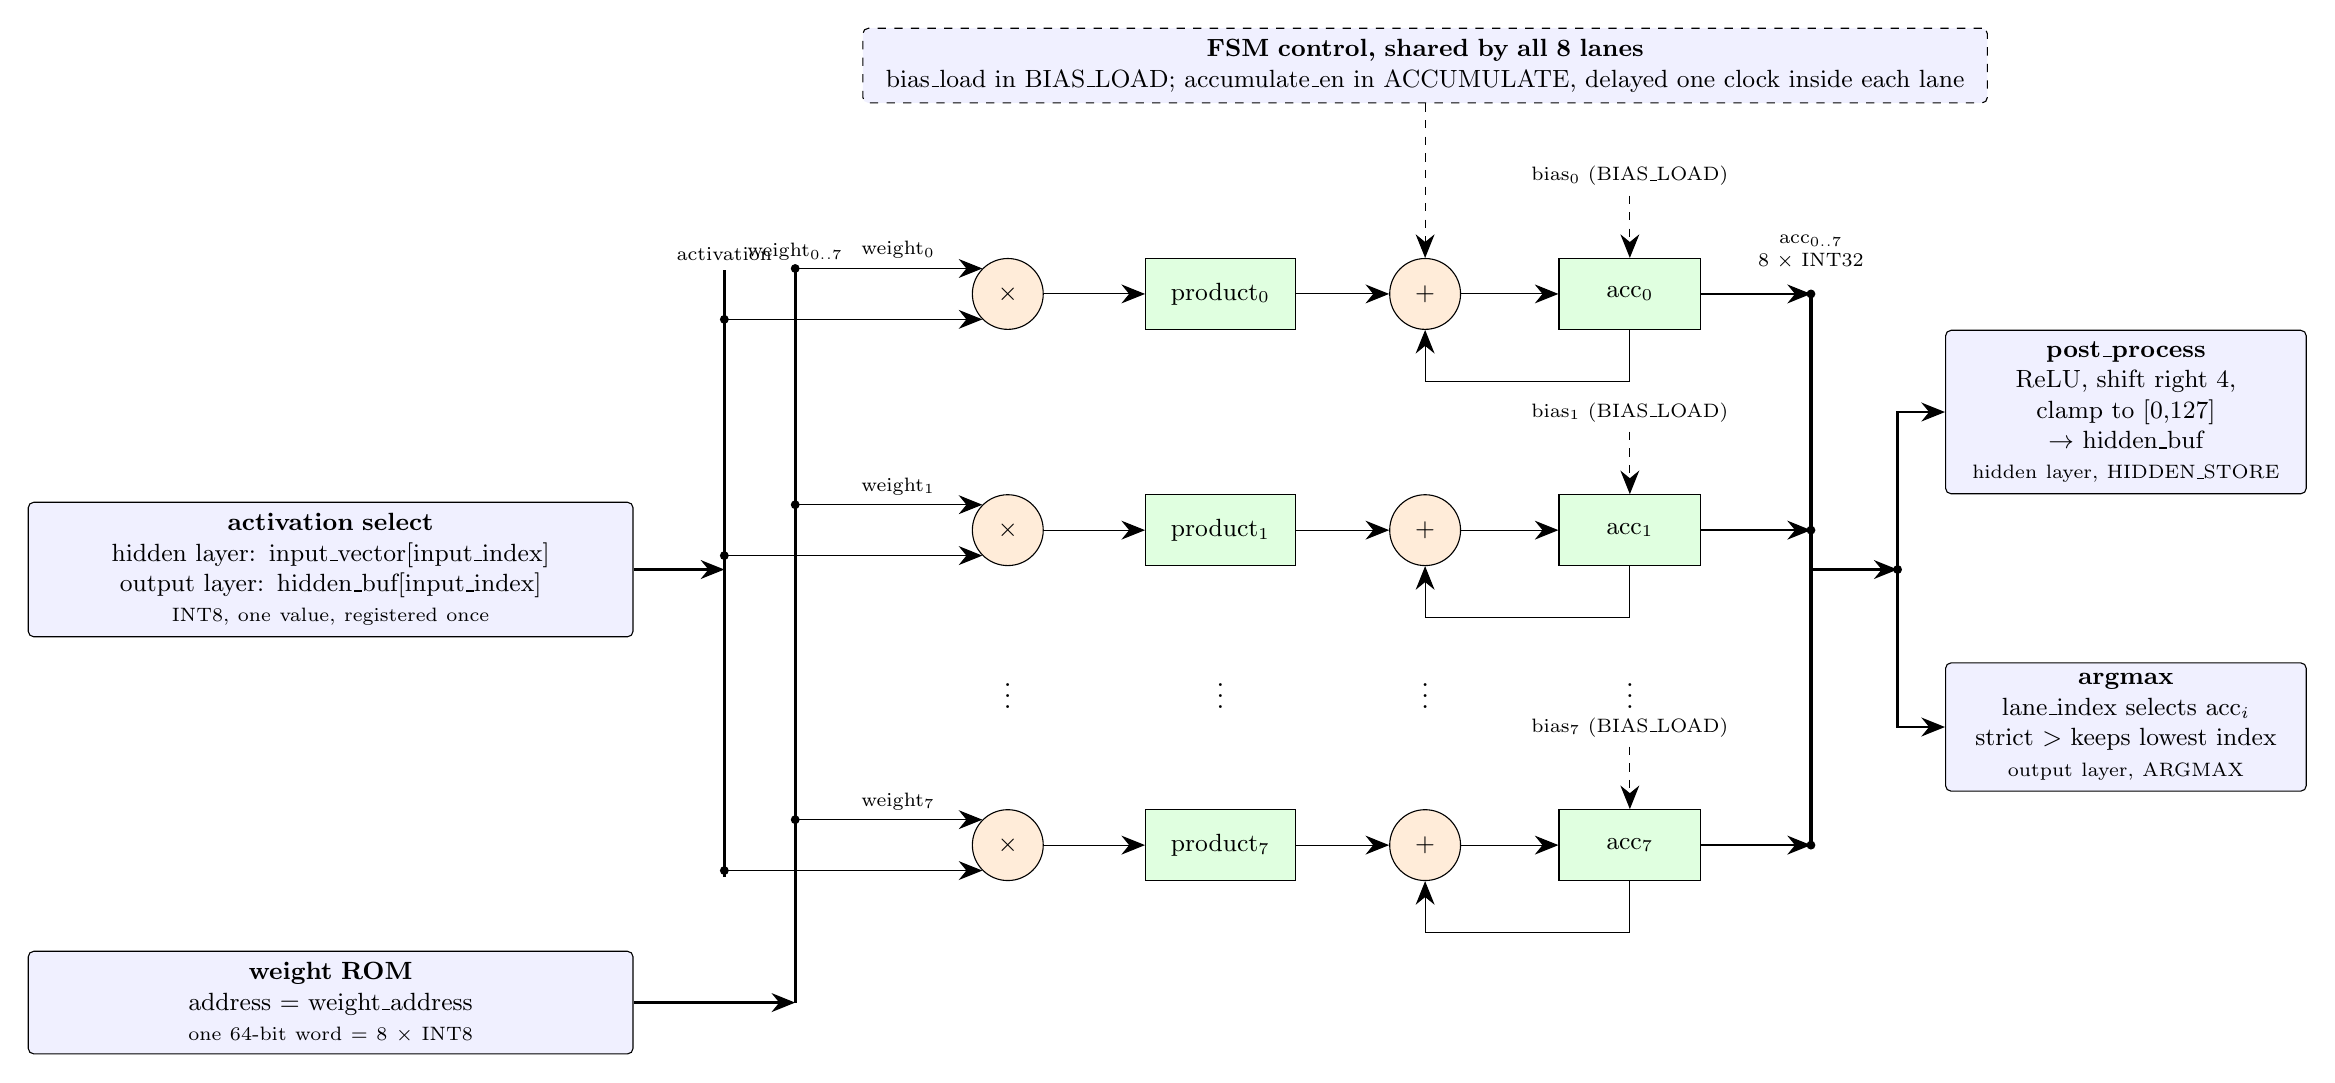
\begin{tikzpicture}[>={Stealth[length=3mm,width=2.4mm]},
  box/.style={draw,rounded corners=2pt,align=center,fill=blue!6,font=\small,inner sep=4pt},
  op/.style={draw,circle,minimum size=0.9cm,fill=orange!15,font=\small},
  reg/.style={draw,minimum width=1.8cm,minimum height=0.9cm,fill=green!12,font=\small},
  bus/.style={very thick}]

\node[box,text width=7.4cm] (actsrc) at (-2.6,-3.5) {\textbf{activation select}\\hidden layer: input_vector[input_index]\\output layer: hidden_buf[input_index]\\{\scriptsize INT8, one value, registered once}};
\node[box,text width=7.4cm] (rom) at (-2.6,-9.0) {\textbf{weight ROM}\\address = weight_address\\{\scriptsize one 64-bit word = 8 $\times$ INT8}};

\draw[bus] (2.4,0.3) -- (2.4,-7.4);
\draw[bus] (3.3,0.3) -- (3.3,-9.0);
\draw[->,thick] (actsrc.east) -- (2.4,-3.5);
\draw[->,thick] (rom.east) -- (3.3,-9.0);
\node[font=\scriptsize,above] at (2.4,0.3) {activation};
\node[font=\scriptsize,above] at (3.3,0.3) {weight$_{0..7}$};

\foreach \y/\i in {0/0,-3.0/1,-7.0/7}{
  \node[op]  (m\i) at (6.0,\y)  {$\times$};
  \node[reg,minimum width=1.9cm] (p\i) at (8.7,\y) {product$_{\i}$};
  \node[op]  (a\i) at (11.3,\y) {$+$};
  \node[reg] (r\i) at (13.9,\y) {acc$_{\i}$};
  \draw[->] (m\i) -- (p\i);
  \draw[->] (p\i) -- (a\i);
  \draw[->] (a\i) -- (r\i);
  \draw[->] (r\i.south) -- ++(0,-0.65) -| (a\i.south);
  \draw[->,dashed] (13.9,\y+1.25) -- (r\i.north);
  \node[font=\scriptsize,above] at (13.9,\y+1.25) {bias$_{\i}$ (BIAS_LOAD)};
  \draw[->] (2.4,0 |- m\i.south west) -- (m\i.south west);
  \fill (2.4,0 |- m\i.south west) circle (1.6pt);
  \draw[->] (3.3,0 |- m\i.north west) -- node[above,pos=0.55,font=\scriptsize]{weight$_{\i}$} (m\i.north west);
  \fill (3.3,0 |- m\i.north west) circle (1.6pt);
  \draw[->,thick] (r\i.east) -- (16.2,\y);
  \fill (16.2,\y) circle (1.6pt);
}
\node at (6.0,-5.0) {$\vdots$};
\node at (8.7,-5.0) {$\vdots$};
\node at (11.3,-5.0) {$\vdots$};
\node at (13.9,-5.0) {$\vdots$};

\draw[bus] (16.2,0) -- (16.2,-7.0);
\node[font=\scriptsize,above,align=center] at (16.2,0.2) {acc$_{0..7}$\\8 $\times$ INT32};

\node[box,text width=4.3cm] (pp) at (20.2,-1.5) {\textbf{post_process}\\ReLU, shift right 4,\\clamp to [0,127]\\$\rightarrow$ hidden_buf\\{\scriptsize hidden layer, HIDDEN_STORE}};
\node[box,text width=4.3cm] (am) at (20.2,-5.5) {\textbf{argmax}\\lane_index selects acc$_i$\\strict $>$ keeps lowest index\\{\scriptsize output layer, ARGMAX}};
\draw[->,thick] (16.2,-3.5) -- (17.3,-3.5);
\draw[->,thick] (17.3,-3.5) |- (pp.west);
\draw[->,thick] (17.3,-3.5) |- (am.west);
\fill (17.3,-3.5) circle (1.6pt);

\node[box,dashed,text width=14cm] (ctl) at (11.3,2.9) {\textbf{FSM control, shared by all 8 lanes}\\bias_load in BIAS_LOAD; accumulate_en in ACCUMULATE, delayed one clock inside each lane};
\draw[->,dashed] (ctl.south) -- (a0.north);
\end{tikzpicture}}
\end{center}

In an ACCUMULATE cycle, lane $i$ multiplies the registered activation by its weight$_i$ and stores the 16-bit product in its product register; one clock later it performs
$\mathit{acc}_i \leftarrow \mathit{acc}_i + \mathit{product}_i$.
The activation (INT8) is registered once and shared by all eight lanes, and weight$_i$ (INT8) is that lane's own slice of the weight word. The weight ROM output is itself registered, so the activation and the weight word meet at the multipliers in the same ACCUMULATE cycle.
The product is INT8 $\times$ INT8 $\to$ 16-bit signed, sign-extended into the 32-bit signed accumulator.
The product register is what lets the multiplier map onto a DSP slice and the design meet 100 MHz; the cost is the DRAIN state, one extra clock after the last input of each group.
In BIAS_LOAD the accumulator is loaded with the lane's 32-bit bias instead of the sum.
The lanes never exchange data with each other, which is what distinguishes this from a systolic array.

\end{landscape}
\end{document}
